\section{The complete compact-correction force and its annulus cost}
\label{ifs:section}

We now evaluate the operation of Proposition~\ref{irc:compact-core-repair}
on its whole support.  Let $I$ be its finite held interval, and choose
$0<r\leq r_c$, with the original $r_c$ and all its material and phase
restrictions retained.  On $B_r$ the actual old fields are
\[
 \theta_h(x,t)=G(t)\cdot x,\qquad u_h(x,t)=A(t)x,\qquad
 p_h(x,t)=\tfrac12 x^TH(t)x,\qquad \operatorname{tr}A=0.
\]
Here $A=A_h,G=G_h,H=H_h$ are the full earlier sums, not selected
components.  Fix a real $\psi\in C_c^\infty(B_1)$ with $\psi=1$ on
$B_{1/2}$, and use $\chi(x)=\psi(x/r)$ in
\eqref{irc:compact-correction}.  Write
$L=\beta\Delta A$, $g=\beta\Delta G$, $K=\beta\Delta H$, and
$B=-JL$, where $J=\left(\begin{smallmatrix}0&-1\\1&0\end{smallmatrix}\right)$.
Then $B$ and $K$ are symmetric and $\operatorname{tr}L=0$.
All coefficients remain time dependent.

\subsection{An exact force map on the complete support}

For an evaluation variable $y=x/r$, define
\begin{align}
 H_g(y)&=\psi(y)\,g\cdot y,&
 q_L(y)&=\tfrac12 y^T(-JL)y,\nonumber\\
 Z_L(y)&=\psi(y)Ly+q_L(y)J\nabla\psi(y),&
 P_K(y)&=\tfrac12\psi(y)y^TKy.
 \label{ifs:cutoff-maps}
\end{align}
These are explicit linear maps of $g,L,K$.  They do not replace the
physical fields: the exact comparison is
\begin{equation}\label{ifs:physical-fields}
 h(ry,t)=rH_{g(t)}(y),\qquad
 z(ry,t)=rZ_{L(t)}(y),\qquad
 \kappa(ry,t)=r^2P_{K(t)}(y).
\end{equation}
In particular $Z_L=J\nabla(\psi q_L)$ and
$\operatorname{div}_yZ_L=0$.
The complete \emph{increment} force is
\begin{align}
 e^\theta(ry,t)
 &=r\mathcal T(y,t)-\frac d r\Delta_y H_g(y),\nonumber\\
 \mathcal T
 &=H_{g'}+(Ay)\cdot\nabla H_g
       +Z_L\cdot G+Z_L\cdot\nabla H_g,
 \label{ifs:scalar-force}\\
 e^u(ry,t)
 &=r\mathcal V(y,t)-\frac d r\Delta_y Z_L(y),\nonumber\\
 \mathcal V
 &=Z_{L'}+AZ_L+(\nabla Z_L)Ay
       +(\nabla Z_L)Z_L+\nabla P_K-H_g e_2.
 \label{ifs:vector-force}
\end{align}
They vanish outside $B_r$.  On $B_{r/2}$ these formulas give exactly
the increment between the old affine residual and
\eqref{irc:transition-scalar}--\eqref{irc:transition-vector}.
The total force everywhere is $f_h+e$; in particular it remains $f_h$
outside $B_r$.  A force estimate for the increment cannot certify a
smaller total force outside that ball.

\begin{proof}
Substitute \eqref{ifs:physical-fields} in the physical subtraction
identities \eqref{ibc:scalar-residual}--\eqref{ibc:vector-residual}.
On the entire support, $u_h(ry)=rAy$,
$\nabla\theta_h=G$ and $\nabla u_h=A$.
One spatial derivative of $rH_g$ or $rZ_L$ removes the factor $r$;
two give $r^{-1}$, whereas $\nabla_x(r^2P_K)=r\nabla_yP_K$.
This gives each displayed term with its shown sign and factor.
All corrections and derivatives vanish near the boundary of $B_r$,
so extension by zero is smooth and the formulas hold globally.
\end{proof}

For example the scalar transport part, with $n=\nabla\psi$, is
\begin{align}
 \mathcal T
 ={}&\psi(g'+A^Tg+L^TG)\cdot y
       +\psi^2 g\cdot Ly+(g\cdot y)n\cdot Ay\nonumber\\
    &+q_L G\cdot Jn+\psi q_Lg\cdot Jn
       +\psi(g\cdot y)n\cdot Ly, \label{ifs:expanded-scalar}\\
 \Delta_yH_g
 ={}&(g\cdot y)\Delta\psi+2g\cdot n. \nonumber
\end{align}
The apparent term $q_L(g\cdot y)(Jn)\cdot n$ is exactly zero
because $J$ is skew symmetric; no other cutoff term was dropped.
For the vector part, put $Q=q_L$, $n=\nabla\psi$,
$S=\nabla^2\psi$ and $k=\tfrac12y^TKy$.  Its full expansion is
\begin{align}
 \mathcal V={}&\psi(L'+AL+LA+K-e_2g^T)y+\psi^2L^2y
       +q_{L'}Jn+QAJn\nonumber\\
 &+(Ly)(n\cdot Ay)+(Jn)((By)\cdot Ay)+QJS\,Ay\nonumber\\
 &+\psi QLJn+\psi(Ly)(n\cdot Ly)
       -Q(n\cdot Ly)Jn\nonumber\\
 &+\psi QJS\,Ly+Q^2JS\,Jn+kn,\label{ifs:expanded-vector}\\
 \Delta_y Z_L={}&(\Delta\psi)Ly+2L\nabla\psi
       +(\operatorname{tr}B)J\nabla\psi
       +2JS\,By+QJ\nabla\Delta\psi. \nonumber
\end{align}
Indeed $(By)\cdot Ly=0$ and $(By)\cdot Jn=-Ly\cdot n$,
as follows from $B=-JL$ and $J^TJ=1$.
These are exact identities retaining strain, pressure, buoyancy,
both quadratic interactions and all diffusion contributions.

\subsection{Every mixed jet and quantitative cutoff constants}

All norms below are Euclidean vector norms, their induced matrix
norms, and supremum norms on $B_1$.
For a multi-index $\gamma\in\mathbb N^2$ set
$\Psi_\gamma=\|\partial^\gamma\psi\|_\infty$ and
$\Phi_\gamma=\|\partial^\gamma\nabla\psi\|_\infty$.
Define the nonnegative constants
\begin{align}
 C^H_\gamma&=\Psi_\gamma+\sum_{j=1}^2
                        \gamma_j\Psi_{\gamma-e_j},\nonumber\\
 Q_\nu&=
 \begin{cases}
 1/2,&|\nu|=0,\\
 1,&1\leq|\nu|\leq2,\\
 0,&|\nu|>2,
 \end{cases}\nonumber\\
 C^Z_\gamma&=C^H_\gamma+
       \sum_{\nu\leq\gamma}\binom\gamma\nu Q_\nu\Phi_{\gamma-\nu},
 \qquad
 C^P_\gamma=\sum_{\nu\leq\gamma}
                   \binom\gamma\nu Q_\nu\Psi_{\gamma-\nu}.
 \label{ifs:constants}
\end{align}
A term with a negative multi-index is zero.
For any such array $C$, put
\[
 (\nabla C)_\gamma=\sum_{j=1}^2 C_{\gamma+e_j},\qquad
 (\Delta C)_\gamma=\sum_{j=1}^2 C_{\gamma+2e_j}.
\]
Let $p_\nu=1$ when $|\nu|\leq1$ and $p_\nu=0$ otherwise, and set
\begin{align}
 \mathfrak A_\gamma(C)
 &=\sum_{\nu\leq\gamma}\binom\gamma\nu
                         p_\nu(\nabla C)_{\gamma-\nu},\nonumber\\
 \mathfrak B_\gamma(C,D)
 &=\sum_{\nu\leq\gamma}\binom\gamma\nu
                         C_\nu(\nabla D)_{\gamma-\nu}.
 \label{ifs:product-constants}
\end{align}
These explicit constants depend only on the selected cutoff and jet,
not on $r,d$ or the parent coefficients.
The product rule and $|y|\leq1$ give
\begin{equation}\label{ifs:linear-map-bounds}
 \|\partial^\gamma H_g\|_\infty\leq C^H_\gamma|g|,
 \quad
 \|\partial^\gamma Z_L\|_\infty\leq C^Z_\gamma\|L\|,
 \quad
 \|\partial^\gamma P_K\|_\infty\leq C^P_\gamma\|K\|.
\end{equation}
To check every factor, derivatives of $g\cdot y$ have orders zero
and one, bounded by $|g|$.  Derivatives of either quadratic
$q_L$ or $y^TKy/2$ have bounds $Q_\nu\|L\|$ or
$Q_\nu\|K\|$, respectively.  Their higher derivatives vanish.
These facts prove \eqref{ifs:constants} term by term.

Write $\mathcal T_{\gamma,b}=\partial_y^\gamma\partial_t^b\mathcal T$
and $\mathcal V_{\gamma,b}=\partial_y^\gamma\partial_t^b\mathcal V$.
Their full signed formulas are
\begin{align}
 \mathcal T_{\gamma,b}
 ={}&\partial^\gamma H_{g^{(b+1)}}\nonumber\\
 &+\sum_{j=0}^b\binom bj\sum_{\nu\leq\gamma}\binom\gamma\nu
   \bigl(\partial^\nu(A^{(j)}y)\bigr)\cdot
          \nabla\partial^{\gamma-\nu}H_{g^{(b-j)}}\nonumber\\
 &+\sum_{j=0}^b\binom bj
       \partial^\gamma Z_{L^{(j)}}\cdot G^{(b-j)}\nonumber\\
 &+\sum_{j=0}^b\binom bj\sum_{\nu\leq\gamma}\binom\gamma\nu
       \partial^\nu Z_{L^{(j)}}\cdot
          \nabla\partial^{\gamma-\nu}H_{g^{(b-j)}},
 \label{ifs:scalar-jets}\\
 \mathcal V_{\gamma,b}
 ={}&\partial^\gamma Z_{L^{(b+1)}}
       +\sum_{j=0}^b\binom bj A^{(j)}
                            \partial^\gamma Z_{L^{(b-j)}}\nonumber\\
 &+\sum_{j=0}^b\binom bj\sum_{\nu\leq\gamma}\binom\gamma\nu
       (\nabla\partial^{\gamma-\nu} Z_{L^{(b-j)}})
                              \partial^\nu(A^{(j)}y)\nonumber\\
 &+\sum_{j=0}^b\binom bj\sum_{\nu\leq\gamma}\binom\gamma\nu
       (\nabla\partial^{\gamma-\nu} Z_{L^{(b-j)}})
                              \partial^\nu Z_{L^{(j)}}\nonumber\\
 &+\nabla\partial^\gamma P_{K^{(b)}}
       -\partial^\gamma H_{g^{(b)}}e_2.
 \label{ifs:vector-jets}
\end{align}
Thus, without interchanging cancellation and norms,
\begin{align}
 (\partial_x^\gamma\partial_t^b e^\theta)(ry,t)
 &=r^{1-|\gamma|}\mathcal T_{\gamma,b}
    -d r^{-1-|\gamma|}\Delta\partial^\gamma H_{g^{(b)}},
 \label{ifs:physical-scalar-jets}\\
 (\partial_x^\gamma\partial_t^b e^u)(ry,t)
 &=r^{1-|\gamma|}\mathcal V_{\gamma,b}
    -d r^{-1-|\gamma|}\Delta\partial^\gamma Z_{L^{(b)}}.
 \label{ifs:physical-vector-jets}
\end{align}
Time derivatives are physical time derivatives here; no clock
factor has been absorbed.

The following computable majorants preserve the complete coefficient
and derivative dependence:
\begin{align}
 T_{\gamma,b}={}&C^H_\gamma|g^{(b+1)}|
  +\sum_{j=0}^b\binom bj\bigl[
    \mathfrak A_\gamma(C^H)\|A^{(j)}\||g^{(b-j)}|\nonumber\\
 &\hspace{24mm}+C^Z_\gamma\|L^{(j)}\||G^{(b-j)}|
    +\mathfrak B_\gamma(C^Z,C^H)\|L^{(j)}\||g^{(b-j)}|\bigr],
 \label{ifs:scalar-majorant}\\
 V_{\gamma,b}={}&C^Z_\gamma\|L^{(b+1)}\|
  +\sum_{j=0}^b\binom bj\bigl[
    (C^Z_\gamma+\mathfrak A_\gamma(C^Z))
                         \|A^{(j)}\|\|L^{(b-j)}\|\nonumber\\
 &\hspace{24mm}+\mathfrak B_\gamma(C^Z,C^Z)
                         \|L^{(j)}\|\|L^{(b-j)}\|\bigr]\nonumber\\
 &+(\nabla C^P)_\gamma\|K^{(b)}\|+C^H_\gamma|g^{(b)}|.
 \label{ifs:vector-majorant}
\end{align}
Consequently the global increment jets satisfy
\begin{align}
 \|\partial_x^\gamma\partial_t^b e^\theta\|_\infty
 &\leq r^{1-|\gamma|}T_{\gamma,b}
       +d r^{-1-|\gamma|}(\Delta C^H)_\gamma |g^{(b)}|,
 \nonumber\\
 \|\partial_x^\gamma\partial_t^b e^u\|_\infty
 &\leq r^{1-|\gamma|}V_{\gamma,b}
       +d r^{-1-|\gamma|}(\Delta C^Z)_\gamma \|L^{(b)}\|.
 \label{ifs:force-majorants}
\end{align}
The Leibniz formulas above prove these inequalities, since a derivative
of $Ay$ has norm at most $\|A\|$ for orders zero or one, and zero
otherwise.  They are sufficient estimates only; the exact signed
expressions \eqref{ifs:physical-scalar-jets}--\eqref{ifs:physical-vector-jets}
are the force being estimated.

\subsection{A quantitative annulus obstruction and its exact defect}

\begin{lemma}\label{ifs:cutoff-diffusion-lower-bound}
The compact cutoff maps satisfy
\[
 \|\Delta H_g\|_\infty\geq2|g|,\qquad
 \|\Delta Z_L\|_\infty\geq2\|L\|.
\]
Their Laplacians are supported in the cutoff annulus
$B_1\setminus B_{1/2}$.
\end{lemma}

\begin{proof}
For a real $f\in C_c^\infty(B_1)$ put
$M=\|\Delta f\|_\infty$ and $w(y)=M(1-|y|^2)/4$.
Since $\Delta w=-M$ in two dimensions, $\Delta(f-w)\geq0$
and $\Delta(-f-w)\geq0$.  Both functions have zero boundary
values.  The maximum principle gives $|f|\leq w\leq M/4$.
Applying this to $H_g$, whose supremum is at least $|g|/2$
on the closed inner ball, proves its bound.
For $L\ne0$, choose a unit vector $v$ with $|Lv|=\|L\|$
and put $a=Lv/\|L\|$.  The scalar $f=a\cdot Z_L$ takes
the value $\|L\|/2$ at $v/2$, so
$\|\Delta Z_L\|_\infty\geq\|\Delta f\|_\infty\geq2\|L\|$.
The zero case is immediate.  On the inner ball the maps are
linear; outside $B_1$ they vanish.  Their Laplacians therefore
have the asserted annular support.
\end{proof}

At every physical time, the \emph{actual signed} force consequently
satisfies
\begin{align}
 \|e^\theta(t)\|_\infty
 &\geq\frac{2d}{r}|g(t)|-r\|\mathcal T(t)\|_\infty
  \geq\frac{2d}{r}|g(t)|-rT_{0,0}(t),\nonumber\\
 \|e^u(t)\|_\infty
 &\geq\frac{2d}{r}\|L(t)\|-r\|\mathcal V(t)\|_\infty
  \geq\frac{2d}{r}\|L(t)\|-rV_{0,0}(t).
 \label{ifs:force-lower-bounds}
\end{align}
This is the reverse triangle inequality, not a claim that diffusion
alone is the force.  In particular a fixed nonzero coefficient
correction at a fixed time, with fixed finite coefficient derivatives,
cannot have an increment force tending to zero merely by letting
$r\downarrow0$.  Its force instead diverges at that time.
The conclusion applies to this precisely specified compact operation.
It does not exclude trajectories whose coefficients or time scales
vary with $r$, or corrections that achieve additional cancellations.

The exact objects which describe the missing cancellation are
\begin{equation}\label{ifs:defect-maps}
 \mathcal D^\theta_r=\frac{r^2}{d}\mathcal T-\Delta H_g,\qquad
 \mathcal D^u_r=\frac{r^2}{d}\mathcal V-\Delta Z_L.
\end{equation}
They are smooth, supported in $B_1$, and satisfy the full morphism
\[
 e^\theta(ry,t)=\frac d r\mathcal D^\theta_r(y,t),\qquad
 e^u(ry,t)=\frac d r\mathcal D^u_r(y,t).
\]
The corresponding mixed-jet map has the exact factor
$d r^{-1-|\gamma|}$ and no time factor.  Thus a bound
$\|\partial_x^\gamma\partial_t^b e\|_\infty\leq\varepsilon$
is \emph{equivalent} to
$\|\partial_y^\gamma\partial_t^b\mathcal D_r\|_\infty
\leq(\varepsilon/d)r^{1+|\gamma|}$, with scalar and vector
components kept separately.
This defines the precise cancellation space for this operation
and its map to the physical all-jet force budget.

The next operation must control these complete defects, retain the
outer parent force, and still realize a subsequent growing return.
The fixed-coefficient localized affine repair does not accomplish
that operation.  Its finite full-support force, every mixed derivative,
and its exact small-force requirement have now been calculated;
the next based return and the infinite smooth-force construction
remain unfinished.  The identities are checked by
\path{full_support_force_check.py} in \path{infinite_modified/checks}.

\begin{figure}[htbp]
 \centering
 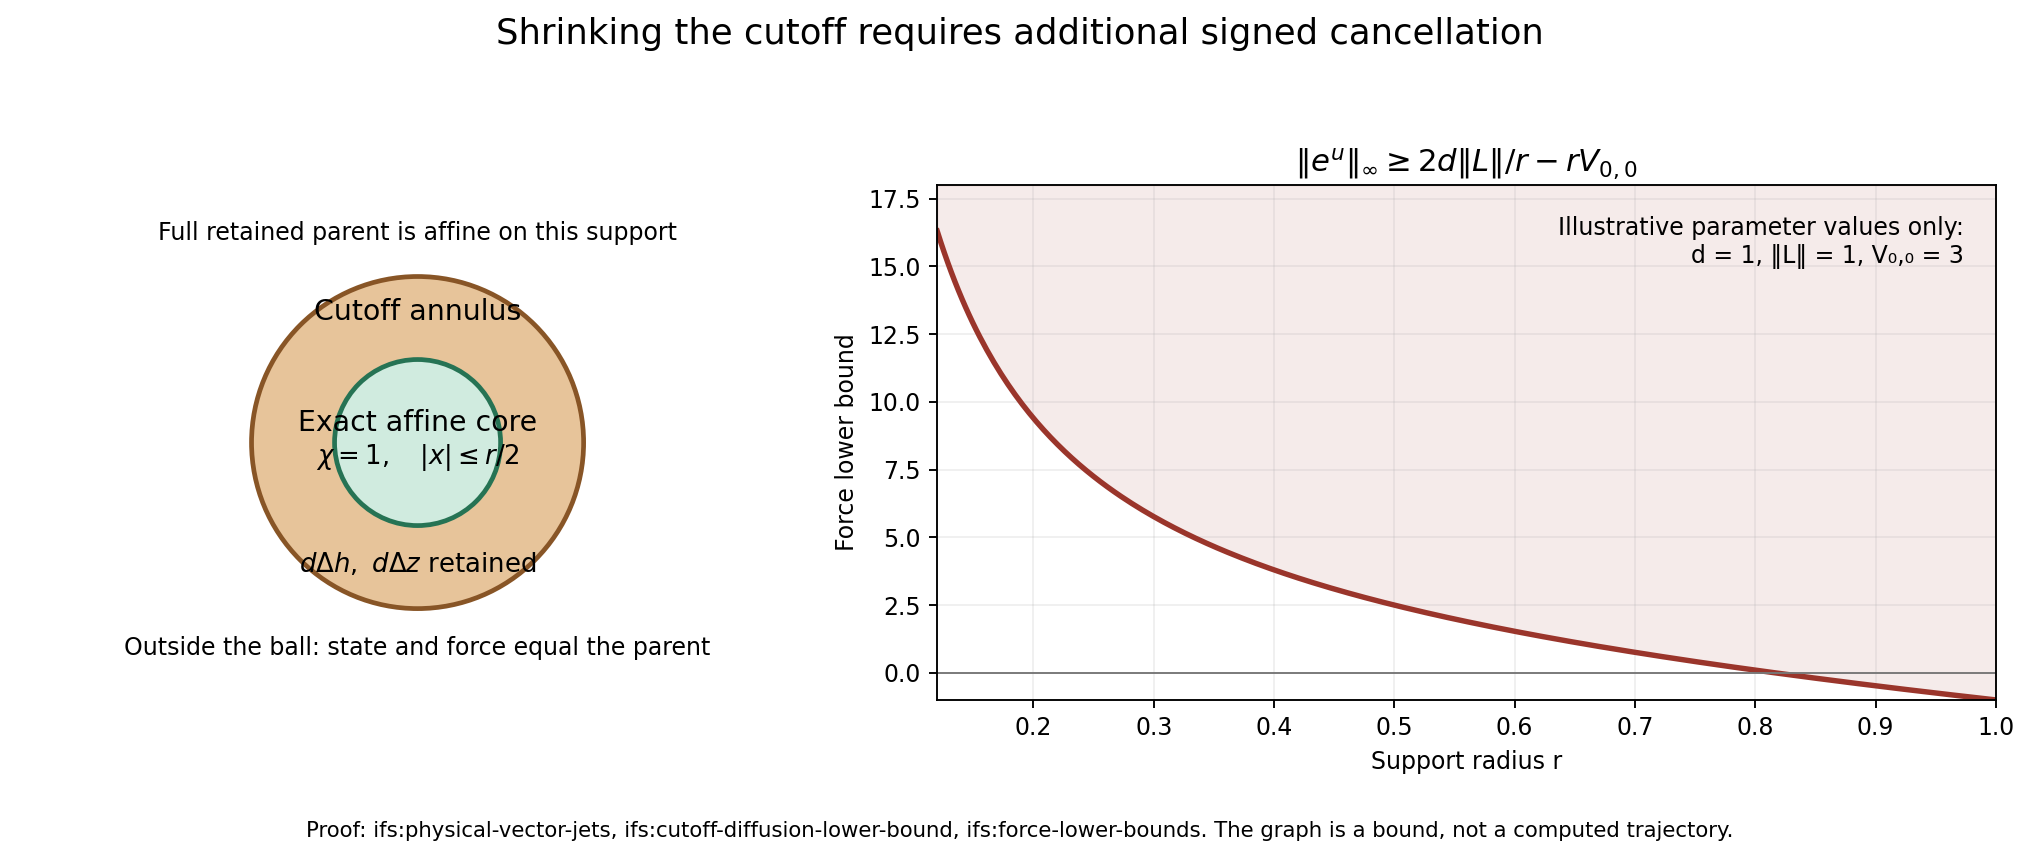
\includegraphics[width=0.97\linewidth]
 {infinite_modified/figures/full_support_force.png}
 \caption{The actual affine parent region permits evaluation of the entire
 compact correction.  Both cutoff Laplacians live in the annulus.
 The graph shows only the proved lower-bound expression at the displayed
 illustrative parameter values, not a sampled solution.  All physical
 diffusion and radius factors remain in the formulas.  The cutoff
 comparison and its proof are \eqref{ifs:physical-fields},
 Lemma~\ref{ifs:cutoff-diffusion-lower-bound} and
 \eqref{ifs:force-lower-bounds}; the source profile is retained from
 Alp\"oge--Buckmaster, Sections 3.3 and 3.7.10.}
 \label{ifs:figure}
\end{figure}
